\documentclass[aspectratio=169, xcolor=table]{beamer}
\usetheme{default}

% --- Packages ---
\usepackage{graphicx}
\usepackage{amsmath,amssymb}
\usepackage{booktabs}
\usepackage{tikz}
\usepackage{array}
\usepackage{multirow}
\usepackage{ragged2e}
\usepackage{animate}

\usetikzlibrary{shapes.geometric, arrows.meta, positioning, calc, fit, backgrounds, decorations.pathreplacing}

% --- Beamer Settings ---
\setbeamertemplate{navigation symbols}{}
\setbeamertemplate{footline}{%
  \hfill%
  \usebeamercolor[fg]{page number in head/foot}%
  \usebeamerfont{page number in head/foot}%
  \insertframenumber\,/\,\inserttotalframenumber%
  \kern1em\vskip1em%
}
\setbeamersize{text margin left=0.55cm, text margin right=0.55cm}

% --- Colors ---
\definecolor{highlightblue}{HTML}{0055A8}
\definecolor{highlightred}{HTML}{E37222}
\definecolor{darkgray}{HTML}{333333}
\definecolor{lightbluefill}{HTML}{EAF2FB}
\definecolor{lightredfill}{HTML}{FBEDE5}
\definecolor{lightgrayfill}{HTML}{F5F5F5}
\definecolor{lightgreenfill}{HTML}{EDF7ED}
\definecolor{hazardred}{HTML}{FF4444}
\definecolor{statenormal}{HTML}{4A90D9}
\definecolor{statequeuing}{HTML}{F5A623}
\definecolor{stateimpacted}{HTML}{D0021B}
\definecolor{statearrival}{HTML}{7ED321}
\definecolor{statesurvival}{HTML}{50C878}
\definecolor{statecasualty}{HTML}{8B0000}

\newcommand{\keyterm}[1]{\textbf{\textcolor{highlightblue}{#1}}}
\newcommand{\source}[1]{\par\vspace{-0.15em}{\raggedleft\fontsize{5.4}{6.0}\selectfont\textcolor{gray}{#1}\par}}
\newcommand{\parambox}[2]{\textcolor{highlightblue}{\textbf{#1}} {\scriptsize--- #2}}

% --- Style ---
\setbeamercolor{title}{fg=highlightblue}
\setbeamercolor{frametitle}{fg=highlightblue}
\setbeamerfont{frametitle}{series=\bfseries,size=\large}
\setbeamerfont{title}{series=\bfseries,size=\Large}
\setbeamercolor{block title}{bg=highlightblue!10, fg=darkgray}
\setbeamercolor{block body}{bg=highlightblue!3, fg=darkgray}
\setbeamercolor{alertblock title}{bg=highlightred!12, fg=darkgray}
\setbeamercolor{alertblock body}{bg=highlightred!4, fg=darkgray}
\setbeamercolor{item}{fg=highlightblue}
\setbeamertemplate{itemize item}{\color{highlightblue}$\blacktriangleright$}
\setbeamertemplate{itemize subitem}{\color{highlightblue}$\bullet$}
\setbeamertemplate{blocks}[rounded][shadow=false]

% --- TikZ styles ---
\tikzset{
  statebox/.style={rounded corners=4pt, minimum width=1.8cm, minimum height=0.85cm,
                   draw=black, thick, text=white, font=\small\bfseries, align=center},
  transarrow/.style={-{Stealth[length=5pt]}, thick, darkgray},
  panelbox/.style={draw=darkgray, rounded corners=6pt, thick, inner sep=6pt},
  flowbox/.style={rounded corners=3pt, minimum width=2.8cm, minimum height=0.6cm,
                  draw=black, thick, font=\scriptsize, align=center},
  flowdiamond/.style={diamond, minimum width=2.2cm, minimum height=1.0cm,
                      draw=black, thick, font=\scriptsize, align=center, inner sep=1pt},
}

% --- Meta ---
\title{Multi-Agent Modeling of Human Traffic Dynamics\\for Rapid Response to Public Emergency\\in Spatial Networks}
\subtitle{Shi, Lee, Yang --- IEEE CASE 2024}
\author{Dalal Alboloushi \quad \& \quad Jeongwon Bae}
\institute{IE 522 --- Simulation \\ Penn State University}
\date{Spring 2026}

\begin{document}

% ============================================================
% SLIDE 1: TITLE
% ============================================================
\begin{frame}[plain]
  \titlepage
\end{frame}

% ============================================================
% SLIDE 2: PROBLEM & MOTIVATION
% ============================================================
\begin{frame}[t,shrink=10]{Problem: Simulating Emergency Evacuation}
\small

\begin{columns}[T,onlytextwidth]
\column{0.55\textwidth}

\textbf{Scenario:} A hazard (fire, explosion, flood) strikes a community.\\
Thousands of pedestrians must evacuate simultaneously.

\vspace{0.6em}
\begin{block}{What makes this hard to simulate?}
\footnotesize
\begin{itemize}\itemsep0.3em
  \item Each person decides \keyterm{independently} --- where to go, which route to take
  \item Decisions depend on \keyterm{local information}: is this road congested? Am I near the hazard?
  \item \keyterm{Panic} causes irrational behavior --- random routing instead of shortest path
  \item Congestion is \keyterm{emergent} --- it arises from many individual decisions, not a global rule
\end{itemize}
\end{block}

\vspace{0.3em}
\begin{alertblock}{}
\footnotesize
A traditional process-flow model cannot capture this.\\
$\Rightarrow$ We need \textbf{Agent-Based Simulation}: model each pedestrian as an autonomous agent with its own state, position, speed, and decision logic.
\end{alertblock}

\column{0.42\textwidth}
\vspace{0.5em}
\begin{center}
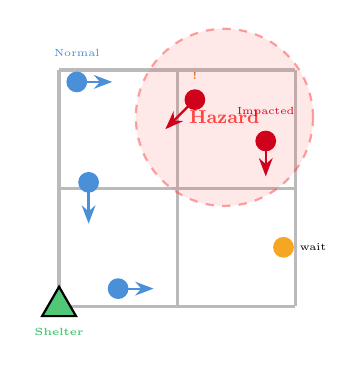
\begin{tikzpicture}[>=Stealth, font=\scriptsize, scale=0.75, transform shape]
  % Simple network
  \draw[lightgrayfill!50!gray, very thick] (0,4) -- (2,4) -- (4,4);
  \draw[lightgrayfill!50!gray, very thick] (0,2) -- (2,2) -- (4,2);
  \draw[lightgrayfill!50!gray, very thick] (0,0) -- (2,0) -- (4,0);
  \draw[lightgrayfill!50!gray, very thick] (0,0) -- (0,2) -- (0,4);
  \draw[lightgrayfill!50!gray, very thick] (2,0) -- (2,2) -- (2,4);
  \draw[lightgrayfill!50!gray, very thick] (4,0) -- (4,2) -- (4,4);

  % Hazard zone
  \fill[hazardred, opacity=0.12] (2.8, 3.2) circle (1.5);
  \draw[hazardred, dashed, thick, opacity=0.5] (2.8, 3.2) circle (1.5);
  \node[hazardred, font=\small\bfseries] at (2.8, 3.2) {Hazard};

  % Agents moving in different directions
  \fill[statenormal] (0.3, 3.8) circle (5pt);
  \draw[->, statenormal, thick] (0.3, 3.8) -- (0.9, 3.8);
  \fill[statenormal] (0.5, 2.1) circle (5pt);
  \draw[->, statenormal, thick] (0.5, 2.1) -- (0.5, 1.4);
  \fill[stateimpacted] (2.3, 3.5) circle (5pt);
  \draw[->, stateimpacted, thick] (2.3, 3.5) -- (1.8, 3.0);
  \node[font=\tiny, highlightred] at (2.3, 3.9) {\textbf{!}};
  \fill[stateimpacted] (3.5, 2.8) circle (5pt);
  \draw[->, stateimpacted, thick] (3.5, 2.8) -- (3.5, 2.2);
  \fill[statenormal] (1.0, 0.3) circle (5pt);
  \draw[->, statenormal, thick] (1.0, 0.3) -- (1.6, 0.3);
  \fill[statequeuing] (3.8, 1.0) circle (5pt);
  \node[font=\tiny] at (4.3, 1.0) {wait};

  % Shelter
  \node[regular polygon, regular polygon sides=3, fill=statesurvival,
        minimum size=0.4cm, draw=black, thick] at (0, 0) {};
  \node[below, font=\tiny\bfseries, statesurvival] at (0, -0.25) {Shelter};

  % Labels
  \node[font=\tiny, statenormal] at (0.3, 4.3) {Normal};
  \node[font=\tiny, stateimpacted] at (3.5, 3.3) {Impacted};
\end{tikzpicture}
\end{center}

\vspace{0.3em}
{\scriptsize\textcolor{gray}{Each dot = one agent making its own decision}}
\end{columns}
\end{frame}

% ============================================================
% SLIDE 3: MODEL OVERVIEW
% ============================================================
\begin{frame}[t]{Model Overview --- Three Components}
\small

\begin{center}
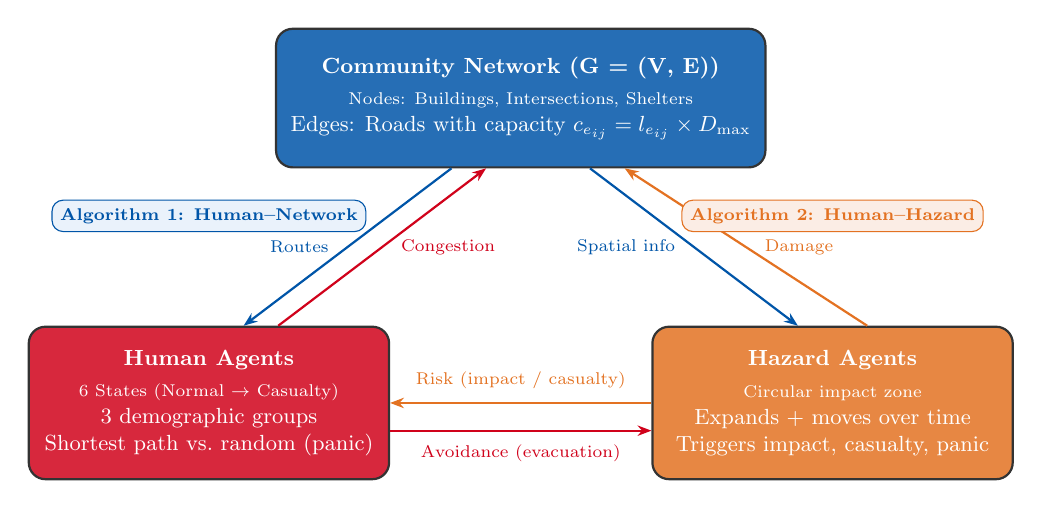
\begin{tikzpicture}[>=Stealth, font=\small, scale=0.88, transform shape]
  % Community Network (top)
  \node[panelbox, fill=highlightblue!85, text=white, minimum width=6.5cm, minimum height=2.0cm, align=center] (net) at (0, 3.2)
    {\textbf{Community Network (G = (V, E))}\\[2pt]
     \scriptsize Nodes: Buildings, Intersections, Shelters\\
     Edges: Roads with capacity $c_{e_{ij}} = l_{e_{ij}} \times D_{\max}$};

  % Human Agents (bottom left)
  \node[panelbox, fill=stateimpacted!85, text=white, minimum width=5.2cm, minimum height=2.2cm, align=center] (human) at (-4.5, -1.2)
    {\textbf{Human Agents}\\[2pt]
     \scriptsize 6 States (Normal $\to$ Casualty)\\
     3 demographic groups\\
     Shortest path vs.\ random (panic)};

  % Hazard Agents (bottom right)
  \node[panelbox, fill=highlightred!85, text=white, minimum width=5.2cm, minimum height=2.2cm, align=center] (hazard) at (4.5, -1.2)
    {\textbf{Hazard Agents}\\[2pt]
     \scriptsize Circular impact zone\\
     Expands + moves over time\\
     Triggers impact, casualty, panic};

  % Left arrows (Network <-> Human)
  \draw[transarrow, highlightblue] ([xshift=-1cm]net.south) -- ([xshift=0.5cm]human.north)
    node[midway, left=4pt, font=\scriptsize, text=highlightblue] {Routes};
  \draw[transarrow, stateimpacted] ([xshift=1cm]human.north) -- ([xshift=-0.5cm]net.south)
    node[midway, right=4pt, font=\scriptsize, text=stateimpacted] {Congestion};

  % Right arrows (Network <-> Hazard)
  \draw[transarrow, highlightblue] ([xshift=1cm]net.south) -- ([xshift=-0.5cm]hazard.north)
    node[midway, left=4pt, font=\scriptsize, text=highlightblue] {Spatial info};
  \draw[transarrow, highlightred] ([xshift=0.5cm]hazard.north) -- ([xshift=1.5cm]net.south)
    node[midway, right=4pt, font=\scriptsize, text=highlightred] {Damage};

  % Bottom arrows (Human <-> Hazard)
  \draw[transarrow, highlightred] (hazard.west) -- (human.east)
    node[midway, above=2pt, font=\scriptsize, text=highlightred] {Risk (impact / casualty)};
  \draw[transarrow, stateimpacted] ([yshift=-4mm]human.east) -- ([yshift=-4mm]hazard.west)
    node[midway, below=2pt, font=\scriptsize, text=stateimpacted] {Avoidance (evacuation)};

  % Algorithm labels
  \node[fill=lightbluefill, rounded corners, draw=highlightblue, font=\scriptsize\bfseries, text=highlightblue] at (-4.5, 1.5) {Algorithm 1: Human--Network};
  \node[fill=lightredfill, rounded corners, draw=highlightred, font=\scriptsize\bfseries, text=highlightred] at (4.5, 1.5) {Algorithm 2: Human--Hazard};
\end{tikzpicture}
\end{center}
\source{Shi et al.\ (2024), Section III}
\end{frame}

% ============================================================
% SLIDE 4: SPATIAL NETWORK --- WHAT IT REPRESENTS
% ============================================================
\begin{frame}[t,shrink=8]{Spatial Network --- What Does It Represent?}
\footnotesize

\begin{columns}[T,onlytextwidth]
\column{0.38\textwidth}
\begin{center}
  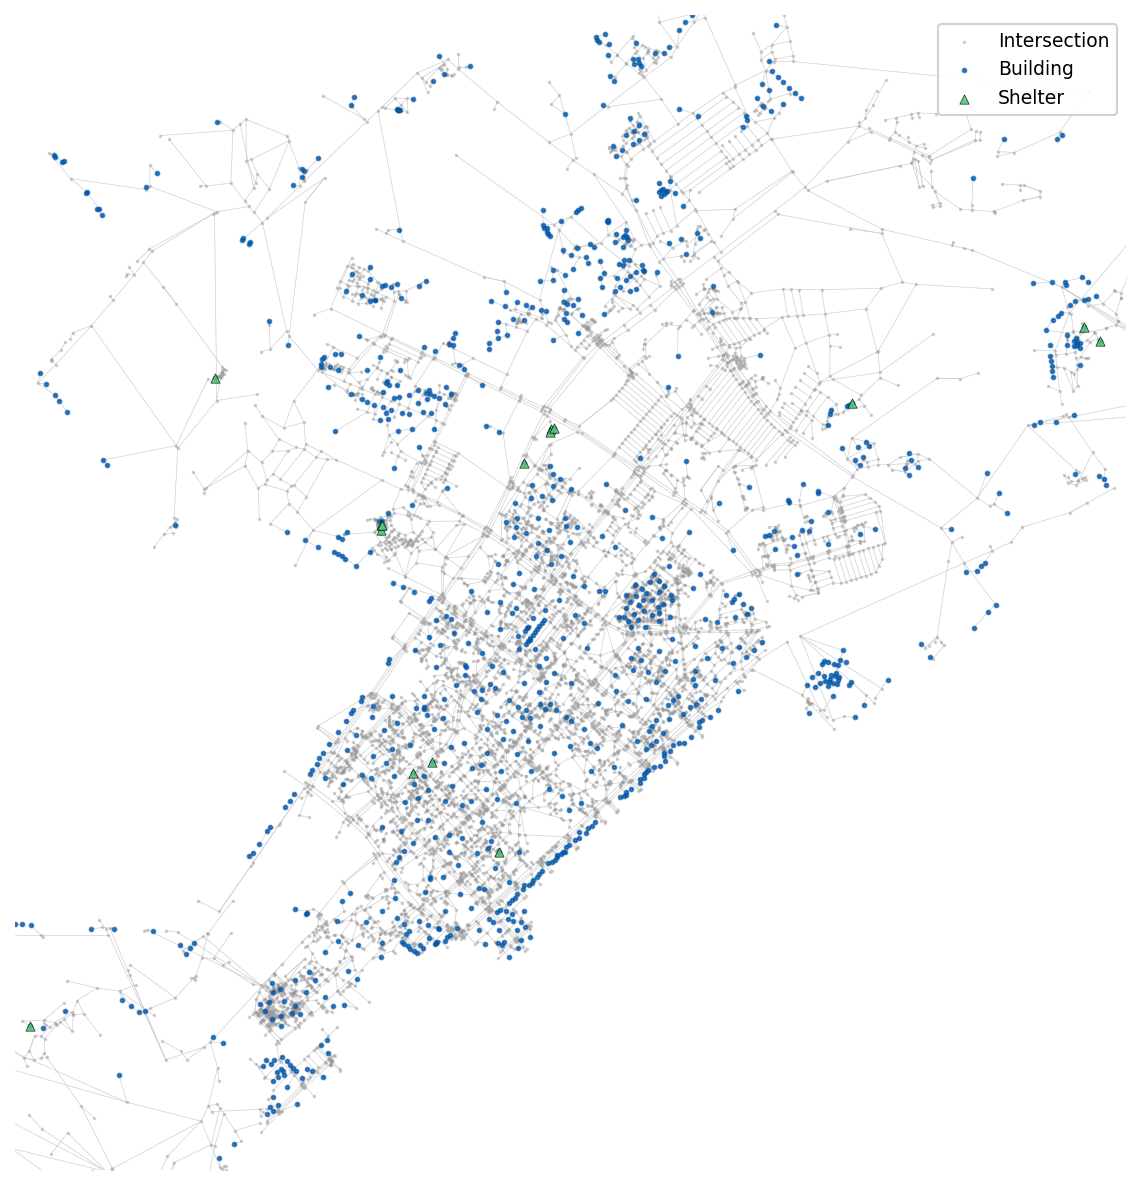
\includegraphics[width=\linewidth]{assets/network_PSU-UP_white.png}\\[2pt]
  {\tiny PSU University Park --- from OpenStreetMap}
\end{center}

\column{0.58\textwidth}
The network is a graph $G = (V, E)$ that represents the \keyterm{physical environment} where evacuation takes place.

\vspace{0.4em}
\begin{block}{Nodes (V) --- Places}
\scriptsize
\begin{itemize}\itemsep0.15em
  \item \textcolor{statenormal}{\textbf{Building nodes}} --- where people start (origins) and go (destinations)
  \item \textbf{Intersection nodes} --- routing decision points
  \item \textcolor{statesurvival}{\textbf{Shelter nodes}} --- safe destinations during emergency
\end{itemize}
\end{block}

\vspace{0.1em}
\begin{block}{Edges (E) --- Roads}
\scriptsize
Each edge has two key properties:
\begin{itemize}\itemsep0.15em
  \item \textcolor{highlightred}{\textbf{Length}} $l_{e_{ij}}$ --- physical distance (meters)
  \item \textcolor{highlightblue}{\textbf{Capacity}} $c_{e_{ij}} = l_{e_{ij}} \times D_{\max}$ --- max pedestrians the road can hold
\end{itemize}
When flow $\geq$ capacity $\Rightarrow$ \textbf{congestion} $\Rightarrow$ agents must queue or reroute.
\end{block}

\vspace{0.1em}
{\scriptsize $D_{\max}$ varies by road type: footway (3), pedestrian zone (8), residential (5) ped/m}
\end{columns}
\source{Shi et al.\ (2024), Section III-A}
\end{frame}

% ============================================================
% SLIDE 5: HUMAN AGENTS --- PARAMETERS & THEIR ROLES
% ============================================================
\begin{frame}[t,shrink=8]{Human Agents --- Parameters \& Their Roles}
\footnotesize

\begin{columns}[T,onlytextwidth]
\column{0.45\textwidth}
\textbf{What defines each agent?}
\vspace{0.2em}

\begin{block}{\scriptsize Core Parameters}
\scriptsize
\begin{itemize}\itemsep0.25em
  \item \parambox{Position}{current node or edge --- ``where am I?''}
  \item \parambox{Destination}{building (normal) or shelter (after impact)}
  \item \parambox{Speed}{how fast they walk (72--96 m/min by age)}
  \item \parambox{State}{behavioral mode --- 6 possible states (right)}
  \item \parambox{Panic rate $\varepsilon_p$}{probability of irrational behavior}
\end{itemize}
\end{block}

\vspace{0.2em}
\begin{alertblock}{\scriptsize What does panic do?}
\scriptsize
\textbf{Normal agent}: computes shortest path to destination each step\\
\textbf{Panicked agent}: picks a \textcolor{highlightred}{random edge} at every node\\[3pt]
$\Rightarrow$ Higher $\varepsilon_p$ = more agents lost = fewer reach shelter
\end{alertblock}

\column{0.52\textwidth}
\textbf{State Transitions}
\vspace{0.1em}

\begin{center}
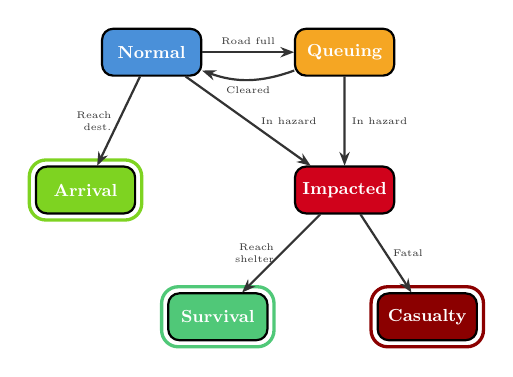
\begin{tikzpicture}[>=Stealth, font=\scriptsize, scale=0.70, transform shape]
  \node[statebox, fill=statenormal] (N) at (0, 3) {Normal};
  \node[statebox, fill=statequeuing] (Q) at (3.5, 3) {Queuing};
  \node[statebox, fill=stateimpacted] (I) at (3.5, 0.5) {Impacted};
  \node[statebox, fill=statearrival] (A) at (-1.2, 0.5) {Arrival};
  \node[statebox, fill=statesurvival] (S) at (1.2, -1.8) {Survival};
  \node[statebox, fill=statecasualty] (C) at (5.0, -1.8) {Casualty};

  \draw[statearrival, very thick, rounded corners=6pt] ([xshift=-3pt, yshift=-3pt]A.south west) rectangle ([xshift=3pt, yshift=3pt]A.north east);
  \draw[statesurvival, very thick, rounded corners=6pt] ([xshift=-3pt, yshift=-3pt]S.south west) rectangle ([xshift=3pt, yshift=3pt]S.north east);
  \draw[statecasualty, very thick, rounded corners=6pt] ([xshift=-3pt, yshift=-3pt]C.south west) rectangle ([xshift=3pt, yshift=3pt]C.north east);

  \draw[transarrow] (N) -- (Q) node[midway, above, font=\tiny] {Road full};
  \draw[transarrow] (Q) to[bend left=20] node[midway, below, font=\tiny] {Cleared} (N);
  \draw[transarrow] (N) -- (A) node[midway, left, font=\tiny, align=right] {Reach\\dest.};
  \draw[transarrow] (N) -- (I) node[midway, right, font=\tiny, xshift=3pt] {In hazard};
  \draw[transarrow] (Q) -- (I) node[midway, right, font=\tiny] {In hazard};
  \draw[transarrow] (I) -- (S) node[midway, left, font=\tiny, align=right] {Reach\\shelter};
  \draw[transarrow] (I) -- (C) node[midway, right, font=\tiny, align=left] {Fatal};
\end{tikzpicture}
\end{center}

\vspace{0.2em}
{\scriptsize
\textbf{Key insight:} Once \textcolor{stateimpacted}{Impacted}, the agent's destination changes from their original building to the \textcolor{statesurvival}{nearest shelter}. Panic is \textbf{irreversible} --- once panicked, the agent never recovers rational routing.}

\end{columns}
\source{Shi et al.\ (2024), Section III-C, Tables II--III}
\end{frame}

% ============================================================
% SLIDE 6: HAZARD AGENTS --- WHAT THEY DO
% ============================================================
\begin{frame}[t,shrink=10]{Hazard Agents --- How Danger Spreads}
\footnotesize

\begin{columns}[T,onlytextwidth]
\column{0.55\textwidth}
\textbf{What defines each hazard?}
\vspace{0.2em}

\begin{block}{\scriptsize Core Parameters}
\scriptsize
\begin{itemize}\itemsep0.3em
  \item \parambox{Center}{starting location on the network}
  \item \parambox{Radius $r(t)$}{how far the danger reaches --- grows over time}
  \item \parambox{Expansion speed}{how fast the radius grows each step}
  \item \parambox{Movement speed}{how fast the center moves}
  \item \parambox{Lifespan}{how long the hazard remains active}
  \item \parambox{Direction}{which way the center drifts}
\end{itemize}
\end{block}

\vspace{0.2em}
\begin{alertblock}{\scriptsize What happens to agents inside the zone?}
\scriptsize
\begin{enumerate}\itemsep0.15em
  \item State $\to$ \textcolor{stateimpacted}{\textbf{Impacted}}, reroute to nearest shelter
  \item Each step: probability of \textcolor{statecasualty}{\textbf{casualty}} (higher near center)
  \item Each step: probability of \textcolor{highlightred}{\textbf{panic}} (irreversible)
\end{enumerate}
\end{alertblock}

\column{0.42\textwidth}
\vspace{0.3em}
\begin{center}
\textbf{Lifecycle:} emergence $\to$ expansion $\to$ movement
\vspace{0.3em}

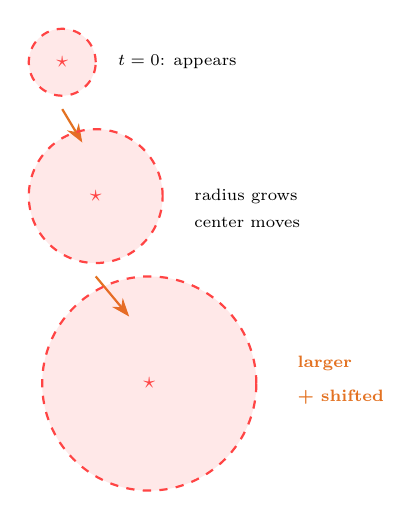
\begin{tikzpicture}[>=Stealth, font=\scriptsize, scale=0.85, transform shape]
  % Stage 1
  \fill[hazardred, opacity=0.12] (1, 3.5) circle (0.5);
  \draw[hazardred, dashed, thick] (1, 3.5) circle (0.5);
  \node[hazardred, font=\normalsize] at (1, 3.5) {$\star$};
  \node[right=6pt, font=\scriptsize] at (1.5, 3.5) {$t=0$: appears};

  % Arrow
  \draw[->, highlightred, thick] (1, 2.8) -- (1.3, 2.3);

  % Stage 2
  \fill[hazardred, opacity=0.12] (1.5, 1.5) circle (1.0);
  \draw[hazardred, dashed, thick] (1.5, 1.5) circle (1.0);
  \node[hazardred, font=\normalsize] at (1.5, 1.5) {$\star$};
  \node[right=10pt, font=\scriptsize] at (2.5, 1.5) {radius grows};
  \node[right=10pt, font=\scriptsize] at (2.5, 1.1) {center moves};

  % Arrow
  \draw[->, highlightred, thick] (1.5, 0.3) -- (2.0, -0.3);

  % Stage 3
  \fill[hazardred, opacity=0.12] (2.3, -1.3) circle (1.6);
  \draw[hazardred, dashed, thick] (2.3, -1.3) circle (1.6);
  \node[hazardred, font=\normalsize] at (2.3, -1.3) {$\star$};
  \node[right=14pt, font=\scriptsize, text=highlightred] at (3.9, -1.0) {\textbf{larger}};
  \node[right=14pt, font=\scriptsize, text=highlightred] at (3.9, -1.5) {\textbf{+ shifted}};
\end{tikzpicture}
\end{center}

\vspace{0.2em}
{\scriptsize\textcolor{gray}{Multiple hazards ($H_{\max}$) can occur during one simulation.}}

\end{columns}
\source{Shi et al.\ (2024), Section III-B}
\end{frame}

% ============================================================
% SLIDE 7: ONE AGENT'S PERSPECTIVE
% ============================================================
\begin{frame}[t,shrink=5]{How It Works --- One Agent's Perspective}
\footnotesize

Each time step (= 1 minute), \textbf{every agent} goes through two checks:

\vspace{0.3em}
\begin{columns}[T,onlytextwidth]
\column{0.48\textwidth}
\begin{alertblock}{\small Step 1: Am I in danger? \normalsize\textcolor{highlightred}{(Algo.\ 2)}}
\scriptsize
\begin{enumerate}\itemsep0.3em
  \item \textbf{Check}: is my position inside any hazard zone?
  \item If \textbf{yes} (first time):
    \begin{itemize}\itemsep0.1em
      \item[$\circ$] State $\to$ \textcolor{stateimpacted}{Impacted}
      \item[$\circ$] New destination $\to$ nearest shelter
    \end{itemize}
  \item If inside zone (every step):
    \begin{itemize}\itemsep0.1em
      \item[$\circ$] Roll for \textcolor{statecasualty}{casualty} (prob.\ $\uparrow$ near center)
      \item[$\circ$] Roll for \textcolor{highlightred}{panic} (prob.\ $= \varepsilon_p \times$ group rate)
    \end{itemize}
  \item If \textbf{no}: skip, proceed to Step 2
\end{enumerate}
\end{alertblock}

\column{0.48\textwidth}
\begin{block}{\small Step 2: Where do I go? \normalsize\textcolor{highlightblue}{(Algo.\ 1)}}
\scriptsize
\begin{enumerate}\itemsep0.3em
  \item \textbf{Check}: am I at my destination?
    \begin{itemize}\itemsep0.1em
      \item[$\circ$] Yes $\to$ \textcolor{statearrival}{Arrival} or \textcolor{statesurvival}{Survival}
    \end{itemize}
  \item \textbf{Check}: is the road ahead full?
    \begin{itemize}\itemsep0.1em
      \item[$\circ$] All edges full $\to$ \textcolor{statequeuing}{Queuing} (wait)
    \end{itemize}
  \item \textbf{Decide route}:
    \begin{itemize}\itemsep0.1em
      \item[$\circ$] \textbf{Not panicked}: recompute shortest path (A*)
      \item[$\circ$] \textbf{Panicked}: pick a random edge
    \end{itemize}
  \item \textbf{Move} along chosen edge at my speed
\end{enumerate}
\end{block}
\end{columns}

\vspace{0.3em}
\begin{center}
\fcolorbox{highlightblue}{lightbluefill}{\parbox{0.85\textwidth}{\centering\scriptsize
\textbf{Simultaneous update}: all agents decide based on the \emph{same} snapshot of the world,\\
then all positions update at once --- no agent has an unfair advantage.
}}
\end{center}
\source{Shi et al.\ (2024), Algorithms 1--2}
\end{frame}

% ============================================================
% SLIDE 8: TOY EXAMPLE
% ============================================================
\begin{frame}[t,shrink=8]{Toy Example --- Simulation in Action}
\footnotesize

\begin{columns}[T,onlytextwidth]
\column{0.50\textwidth}
\vspace{0.1em}
\begin{center}
\animategraphics[controls,loop,width=0.95\linewidth]{3}{assets/frames/frame_}{000}{027}
\end{center}

\column{0.46\textwidth}
\vspace{0.1em}

\textbf{Timeline}
\vspace{0.2em}

\begin{block}{\scriptsize $t = 0$\,: Normal operation}
\scriptsize
10 agents depart from \textcolor{statenormal}{\textbf{buildings}} toward random destinations.
\end{block}

\begin{alertblock}{\scriptsize $t = 4$\,: Hazard emerges}
\scriptsize
Agents in the zone $\to$ \textcolor{stateimpacted}{\textbf{Impacted}}, reroute to \textcolor{statesurvival}{\textbf{shelter}}.\\
Some become \textcolor{statecasualty}{\textbf{casualties}} ($\times$).
\end{alertblock}

\begin{block}{\scriptsize $t = 10\text{--}25$\,: Evacuation under pressure}
\scriptsize
\begin{itemize}\itemsep0.1em
  \item Zone expands $\to$ more agents impacted
  \item \textcolor{statequeuing}{\textbf{Queuing}} at congested edges
  \item \textcolor{highlightred}{\textbf{Panicked}} agents (!) walk randomly
  \item Others follow shortest path to shelter
\end{itemize}
\end{block}

\begin{block}{\scriptsize $t = 25$\,: Evacuation complete}
\scriptsize
All agents resolved: Arrival, Survival, or Casualty.\\
Hazard zone still active but no one left inside.
\end{block}

\end{columns}
\end{frame}

% ============================================================
% SLIDE 9: CURRENT STATUS & PROJECT DIRECTION
% ============================================================
\begin{frame}[t,shrink=8]{Current Status \& Project Direction}
\footnotesize

\begin{columns}[T,onlytextwidth]
\column{0.42\textwidth}

\begin{block}{\small What we have done}
\scriptsize
\begin{itemize}\itemsep0.2em
  \item[$\checkmark$] Paper analysis \& model understanding
  \item[$\checkmark$] Base implementation complete\\
        {\tiny (network, agents, hazards, Algorithms 1--2)}
  \item[$\checkmark$] Toy simulator with all 6 states,\\
        congestion, panic, simultaneous update
  \item[$\circ$] Validation against paper: \textbf{pending}
\end{itemize}
\end{block}

\vspace{0.1em}
\begin{alertblock}{\small Reproduction targets}
\scriptsize
\begin{itemize}\itemsep0.2em
  \item \textbf{Table V:} Verify network structure\\
        (Buildings, Non-building nodes, Edges)\\
        for 5 communities:\\
        {\tiny PSU Univ.\ Park, UVA Charlottesville, Virginia Tech,
        Reading PA, King of Prussia PA}

  \item \textbf{Fig.\ 5:} Impacted Rate (RI) vs.\ max pedestrian flow ($P_{\max}$), grouped by number of hazard events ($H_{\max}$)

  \item \textbf{Fig.\ 6:} Survival / Casualty / Leftover Rates vs.\ Panic Rate ($\varepsilon_p$)
\end{itemize}
\vspace{0.1em}
{\tiny 45 parameter combinations ($3 \times 3 \times 5$), multi-seed averaging}
\end{alertblock}

\column{0.54\textwidth}

\begin{block}{\small Reproduction approach}
\scriptsize
\begin{itemize}\itemsep0.2em
  \item Build identical walk networks from OpenStreetMap for each community
  \item Run full factorial experiment:\\
        $P_{\max} \in \{2000, 5000, 8000\}$\\
        $H_{\max} \in \{5, 10, 15\}$ (number of hazard events)\\
        $\varepsilon_p \in \{10\%, 30\%, 50\%, 70\%, 90\%\}$
  \item Compare quantitatively with the paper's published Table~V, Fig.~5, and Fig.~6
\end{itemize}
\end{block}

\vspace{0.1em}
\begin{alertblock}{\small Future work (from the paper's discussion)}
\scriptsize
\begin{itemize}\itemsep0.2em
  \item \textbf{Additional agent types:}\\
        Add firefighters, trained volunteers\\
        to model organized response alongside evacuation
  \item \textbf{Social force models:}\\
        More realistic panic behavior using\\
        physics-based crowd dynamics (attraction/repulsion)
  \item \textbf{Markov Decision Processes:}\\
        Probabilistic modeling of irrational decisions\\
        triggered by evolving hazard conditions
\end{itemize}
\end{alertblock}

\end{columns}
\end{frame}

\end{document}
